% !TeX root = ../main.tex
% Add the above to each chapter to make compiling the PDF easier in some editors.

\chapter{Methodik}\label{chapter:Methodik}
%Kurz erklären, warum Hypothesen aufstestellt wurden. Und wofür die Skala oder Diagramm, je nachdem was es wird dienen soll.

\section{Hypothesen}\label{section:Hypothesen}
Anhand der vorausgegangenen Literaturrecherche kann eine Vielzahl an Hypothesen bezüglich Situationen und Eigenschaften, die ein höheres Unfallrisiko mit sich bringen aufgestellt werden. Im Rahmen dieser Arbeit werden Hypothesen aufgestellt, die später mit den vorliegenden Unfalldaten verglichen und auf ihre Gültigkeit überprüft werden. Im Fokus vieler Unfallforschungen steht vielmals das Alter oder die Aufmerksamkeit der Unfallbeteiligten, ebenso spielt die Geschwindigkeitsüberschreitung häufig eine wichtige Rolle. Diese Punkte werden hier nicht weiter beachtet, da sie bei den vorhandenen Unfalldaten nicht gegeben sind. Des weiteren wird der Einfluss von berauschenden Mitteln nicht weiter analysiert. Dieser Punkt wird vernachlässigt, da später kritische Situationen mit einem menschlichen Fahrer, mit automatisierten Fahrsituationen verglichen werden sollen. Der Zustand des Fahrers ist beim vollautomatisierten Fahren nicht von Bedeutung und wird im Folgenden nicht weiter berücksichtigt. Um Unfälle kritischen Fahrsituationen zuordnen zu können muss man die Unfälle detailliert betrachten. Der Unfalltyp allein reicht dafür z.B. nicht aus. Deshalb sind auch die Hypothesen zum Teil sehr spezifisch und orientieren sich größtenteils an beim Unfall von der Polizei angegebenen Unfallursachen.

Das innerstädtische Straßennetz wird von Knotenpunkten geprägt, an denen viele verschiedene Fahrsituationen auftreten. Bei Abbiegevorgängen handelt es sich dabei um Situationen die viele Konfliktpunkte aufweisen. Es wir angenommen, dass:

\begin{itemize}
	\item Bei der Fahrsituation Linksabbiegen im Vergleich zur Situation Abbiegen nach rechts mehr Konfliktpunkte auftreten. Daher kommt es beim Linksabbiegen häufiger zu Unfällen. (\textit{Hypothese 1})
	\item Die Konfliktpunkte und Unfallzahlen können reduziert werden, wenn Linksabbieger, an Kreuzungen mit LSA, auf einem eigenen Fahrstreifen mit eigener Signalphase geführt werden. (\textit{Hypothese 2})
\end{itemize}

Es kommt im urbanen Raum jedoch nicht nur zu Unfällen durch Abbiegemanöver. Vor allem bei dichtem Verkehr dürfen Unfälle im Längsverkehr und mit Fahrzeugen im ruhenden Verkehr nicht vernachlässigt werden. 

\begin{itemize}	
	\item Bei höherem Verkehrsaufkommen, z.B. in den Hauptverkehrszeiten, steigt die Anzahl der Verkehrsunfälle im Längsverkehr. Ursachen dafür sind Konflikte beim Spurwechsel und zu geringer Sicherheitsabstand. (\textit{Hypothese 3})
	\item Im urbanen Raum kommt es häufig zu Konflikten mit Fahrzeugen im ruhenden Verkehr. Besonders auffällig sind Bereiche mit Längsaufstellung am Fahrbahnrand. Zusätzlich spielt verbotswidriges auf der Straße Halten/Parken, z.B. Parken in zweiter Reihe, eine bedeutende Rolle. Beim Vorbeifahren entstehen kritische Situationen die zu Unfällen führen. (\textit{Hypothese 4})
\end{itemize}

Urbane Fahrsituationen werden zusätzlich von nicht motorisierten Verkehrsteilnehmern beeinflusst. Hierbei muss berücksichtigt werden, dass:
	
\begin{itemize}
	\item Die Komplexität einer Fahrsituation und somit auch die Zahl der Unfälle wird erhöht, wenn nicht motorisierte Verkehrsteilnehmer daran beteiligt sind. Durch den geringen Schutz von Radfahrern/Fußgängern ist der Verletzungsgrad höher als bei Unfällen, an denen nur motorisierte Verkehrsteilnehmer beteiligt sind. (\textit{Hypothese 5})
	\item Wenn sich Fußgänger und Radfahrer parallel zum Fahrzeug bewegen kommt es beim Rechtsabbiegen häufiger zu Unfällen als beim Linksabbiegen. Kritische Situationen treten vor allem dann auf, wenn Radfahrer den Radweg in die falsch Richtung befahren. (\textit{Hypothese 6})
	\item Bei baulich von der Fahrbahn getrennten Radverkehrsanlagen kommt es häufiger zu Unfällen als bei Radverkehrsanlagen auf der Fahrbahn. Die Unfallgefahr wird durch schlechte bzw. nicht vorhandene Markierungen der Radverkehrsanlagen, besonders im Bereich von Knotenpunkten, erhöht. (\textit{Hypothese 7})
	\item Falsches Verhalten der Fußgänger ist häufig die Ursache für Unfälle mit Personenschaden im urbanen Raum. Besonders häufig treten die Ursachen Rotlichtverstöße und Überschreiten der Fahrbahn ohne auf den Fzg.-Verkehr zu achten auf. Häufig ereignen sich solche Unfälle in der Nähe von Haltestellen des ÖPNV's. (\textit{Hypothese 8})
\end{itemize}	

Neben den Unfallursachen, die Fahrzeugführern oder Fußgängern zugeschrieben werden können gibt es auch noch allgemeine Ursachen die von den Straßenverhältnissen, Witterungseinflüssen oder Hindernissen im Straßenraum beeinflusst werden. Hier kommt es vor allem 

\begin{itemize}	
	\item Bei Sichtbehinderungen durch Witterungseinflüsse bei der Unfallursache "Blendende Sonne" vermehrt zu Unfällen. (\textit{Hypothese 9})
\end{itemize}

Die hier aufgeführten Hypothesen werden in Kapitel \ref{sechtion:Überprüfung der Thesen} anhand der Unfalldaten des Testgebiets überprüft. Hier soll jedoch schon darauf hingewiesen werden, dass die Ergebnisse aufgrund der eher geringen Unfallzahlen im Testgebiet und teilweise unvollständigen Daten nicht auf andere Bereiche übertragbar sind. % Kann man das so stehen lassen?


\section{Bewertung urbaner Fahrsituationen}\label{section:Bewertung urbaner Fahrsituationen}
Unfälle im urbanen Raum treten nicht nur häufig auf, ihnen liegen auch viele verschiedene Fahrsituationen zugrunde. Hierbei gibt es Situationen die ein erhöhtes Risiko aufweisen, wenn sich ein Unfall ereignet und solche, denen eher ein geringes Risiko zugeordnet wird. Eine Bewertungsskala ist hilfreich, Unfälle bzw. Fahrsituationen bezüglich ihrer Sicherheitsrelevanz zu klassifizieren. Deshalb wird in diesem Kapitel, basierend auf den Ergebnissen aus Kapitel \ref{section:Ansätze zur Bewertung von Fahrsituationen}, eine Methode zur Bewertung von urbanen Fahrsituationen entwickelt.

\subsection{Vorgehen zur Typisierung von Unfällen}\label{subsection:Vorgehen zur Typisierung}
Der vorhandene, von der Polizei aufgenommene Datensatz, enthält unterschiedlich ausführliche Angaben. Zu Unfällen, bei denen sich ein Personenschaden oder ein schwerwiegender Sachschaden im engeren Sinne ereignete, liegen ausführlichere Informationen vor, als zu denjenigen die nicht in diese beiden Kategorien passen. Liegen weniger ausführliche Angeben vor handelt es sich um eine Kurzaufnahme eines Unfalls. Diese Unfälle werden im folgenden als Kleinunfall bezeichnet. Bei einer Kurzaufnahme werden lediglich Datum, Uhrzeit, Ort und Allgemeine Ursachen des Unfalls im Aufnahmeformular angegeben. Anhand dieser Informationen lässt sich der Unfallhergang jedoch nur schwer nachvollziehen. Hierfür eigenen sich Beschreibungen des Unfalls. Diese wurden nachträglich bei der Polizei München angefragt. Aufgrund von Datenschutzgründen konnten jedoch nur noch Beschreibungen (Kurzsachverhalte) für die Jahre 2013 bis 2016 zur Verfügung gestellt werden. Die für das Jahr 2012 wurden bereits gelöscht. Daher wird bei der Typisierung der Unfälle und der folgenden Bewertung, in Kapitel \ref{section:Zuordnung der Unfälle zu Fahrsituationen}, nur ein Datensatz über vier Jahre berücksichtigt.

Die Unfälle, die sich im Testgebiet ereigneten, sollen Typisiert werden um die Häufigkeit eines bestimmten Unfalltyps zu bestimmen. Hierfür kann man zunächst die sieben Unfalltypen verwenden. Diese sind jedoch sehr allgemein gehalten. Es wird z.B. nur angegeben, dass es sich um einen Abbiege-Unfall handelt. Unklar ist ob dieser sich beim Abbiegen nach rechts oder nach links ereignet hat und wer an dem Unfall beteiligt war. Deshalb werden hier die Unfalltypen nach GDV herangezogen, sie wurden z.T. bereits in Kapitel \ref{section:urbane Fahrsituationen und ihre Sicherheitsbewertung} vorgestellt. Alle Feintypen sind im  Anhang \ref{chapter:Anhang1} dargestellt.

Bei dieser Arbeit wird zunächst den Unfällen ein Feintyp zugeordnet, bei denen bereits ein Unfalltyp angegeben wurde (keine Kleinunfälle). Hierfür werden die Kurzsachverhalte einzeln durchgearbeitet und mit den Angaben im Unfallprotokoll verglichen. Bei sich widersprechenden Angaben wird die Angaben der Kurzsachverhalte herangezogen. Wurde bei einem Unfall z.B. der Unfalltyp Abbiege-Unfall angegeben, in der Kurzbeschreibung wurde jedoch ein Unfall beschrieben, bei dem es zu einem Zusammenstoß mit einem von links kommenden Fahrzeug und einem Rechtsabbieger kommt, wird dem Unfall der Feintyp 303 (siehe Abbildung \ref{fig:Einbiege-Unfall}) zugeordnet.

Anschließend werden die Kleinunfälle betrachtet. Hier sind in erster Linie die Kurzsachverhalte für die Zuordnung der Feintypen relevant. Sie werden zusätzlich mit der angegebenen Allgemeinen Ursache und dem Unfallort abgeglichen. Hierfür werden die Kurzsachverhalte wieder einzeln durchgearbeitet. Bei einem Unfall wurde z.B. folgendes angegeben: \enquote{Zum Unfallzeitpunkt befuhr die 02 die Rheinstraße in östlicher Richtung. An der Kreuzung Rheinstraße/Leopoldstraße wollte die 02 nach links in die Leopoldstraße abbiegen. Dazu ordnete sie sich auf der Linksabbiegerspur ein. Auch die 01 hatte dieselbe Absicht und befuhr hinter der 02 die Linksabbiegerspur. Bei grünem Licht der LZA fuhr die 02 in den Kreuzungsbereich ein, musste verkehrsbedingt bremsen. 01 konnte ihren Wagen nicht mehr zum Stillstand bringen und fuhr mangels Sicherheitsabstandes auf den Pkw der 02 auf.} Hierbei handelt es sich um einen Unfall dem der Feintyp 201 in Abbildung \ref{fig:Abbiege-Unfall} zugeordnet wird.

Teilweise sind die Beschreibungen sehr kurz gehalten und geben keine detaillierte Auskunft. Es ist daher mit dieser Methode nicht möglich, alle Unfälle mit Feintypen zu typisieren. Die Anzahl der Unfälle denen kein Feintyp zugeordnet werden kann ist jedoch gering. Es ist sehr aufwendig, alle Kurzsachverhalte durchzulesen. Daher ist es denkbar für größere Datensätze, den Feintypen Wortgruppen zuzuordnen, nach denen dann gefiltert wird. Diese Methode wurde hier nicht angewendet. % Evtl noch mehr dazu schreiben?

\subsection{Bewertungsskala}\label{subsection:Bewertungsskala}
Die Unfälle innerhalb des Testgebiets sollen bezüglich ihrer Sicherheitsrelevanz bewertet werden. Hierfür werden zunächst die Unfälle betrachtet, denen bei der Unfallaufnahme ein Unfalltyp zugeordnet wurde. Im weiteren Verlauf wird die Häufigkeit der typisierten Unfälle berechnet. Durch die Typisierung fließen nun auch die Kleinunfälle mit in die Berechnung ein, die gesamte Anzahl der Unfälle nimmt daher deutlich zu. Zuerst werden wieder nur die sieben Unfalltypen betrachtet, dann wird die Anzahl der Unfälle mit einem bestimmten Feintyp auf die gesamte Anzahl der Unfälle im Testgebiet bezogen. Bei der Gesamtanzahl wird zwischen zwei Fällen unterschieden. Der Erste betrachtet nur die Unfälle die ausführlich aufgenommen wurden, bei denen es also zu einem Personenschaden oder Sachschaden im engeren Sinne kam, siehe Formel \ref{equation:Häufigkeit(1)}. Der Zweite dagegen berücksichtigt alle Unfälle im gesamten Untersuchungsgebiet (Formel \ref{equation:Häufigkeit(2)} und \ref{equation:Häufigkeit(3)}).

\begin{equation}\label{equation:Häufigkeit(1)}
\text{Häufigkeit(x)} = \dfrac{\text{Anzahl Unfälle mit Unfalltyp x}}{\text{Anzahl Unfälle mit P \& S}}*100
\end{equation}

\begin{equation}\label{equation:Häufigkeit(2)}
\text{Häufigkeit(x)} = \dfrac{\text{Anzahl Unfälle mit Unfalltyp x}}{\text{Anzahl Unfälle gesamt}}*100
\end{equation}

\begin{equation}\label{equation:Häufigkeit(3)}
\text{Häufigkeit(x)} = \dfrac{\text{Anzahl Unfälle mit Feintyp x}}{\text{Anzahl Unfälle gesamt}}*100
\end{equation}

Die Anzahl der Unfälle für die Jahre 2013 bis 2016 haben im Testgebiet folgende Werte:

\begin{itemize}
	\item Anzahl Unfälle mit P \& S = 591 Stück
	\item Anzahl Unfälle gesamt = 1779 Stück
\end{itemize}

Die so berechnete Häufigkeit der einzelnen Unfalltypen bzw. Feintypen wird nun einem gewissen Bereich der Eintrittswahrscheinlichkeit zugeordnet. Hierfür stehen die vier Bereiche \textit{sehr selten}, \textit{selten}, \textit{oft} und \textit{sehr oft} zur Verfügung. Dieses Vorgehen orientiert sich an dem Risikograph nach DIN V 19250, welcher in Kapitel \ref{subsection:Risikograph} vorgestellt wird. Um eine sinnvolle Einteilung der  vier Bereiche zu erhalten erfolgt dies jeweils unter Berücksichtigung der Anzahl der verschiedenen Unfalltypen bzw. Feintypen und der gesamten Anzahl der Unfälle. Tabelle \ref{tab:Haeufigkeits Bereiche} stellt die Eintrittsbereiche dar, die im Verlauf der Arbeit, auf die drei oben genannten Fälle, angewendet werden.

\begin{table}[htpb]
	\scriptsize
	\caption[Eintrittswahrscheinlichkeit der Unfälle im Testgebiet, bei der Betrachtung von Unfalltypen und Feintypen]{Eintrittswahrscheinlichkeit der Unfälle im Testgebiet, bei der Betrachtung von Unfalltypen und Feintypen}\label{tab:Haeufigkeits Bereiche}
	\centering
	\begin{tabular}{l l l  l l}
		\toprule
		Fall & sehr selten & selten & oft & sehr oft \\
		\midrule
		Unfalltypen für S \& P & 0 \% < 7 \%  & 7 \% < 14 \% & 14 \% < 21 \% & 21 \% < 28 \%\\
		Unfalltypen mit K & 0 \% < 11 \%  & 11 \% < 22 \% & 22 \% < 33 \% & 33 \% < 44 \%\\
		Feintypen & 0 \% < 0,5 \% & 0,5 \% < 1,5 \% & 1,5 \% < 3 \% & 3 \% < 8 \%\\
		\bottomrule
	\end{tabular}
\end{table}

Bis jetzt wurden die Unfälle nur Anhand der Häufigkeit ihres Auftretens bewertet. Es sind jedoch nicht nur die Unfälle sicherheitsrelevant, welche am Häufigsten vorkommen, sondern auch solche, die schwere Folgen haben. Besonders kritisch sind Unfälle die häufig auftreten und zu schweren Folgen führen. Deshalb wird zusätzlich die Unfallschwere angegeben. Aus den oben genannten Formeln ergeben sich nun die Formeln \ref{equation:Häufigkeit(4)}, \ref{equation:Häufigkeit(5)} und \ref{equation:Häufigkeit(6)}.

\begin{equation}\label{equation:Häufigkeit(4)}
\text{Häufigkeit(xy)} = \dfrac{\text{Anzahl Unfälle mit Unfalltyp x und Unfallschwere y}}{\text{Anzahl Unfälle mit P \& S}}*100
\end{equation}

\begin{equation}\label{equation:Häufigkeit(5)}
\text{Häufigkeit(xy)} = \dfrac{\text{Anzahl Unfälle mit Unfalltyp x und Unfallschwere y}}{\text{Anzahl Unfälle gesamt}}*100
\end{equation}

\begin{equation}\label{equation:Häufigkeit(6)}
\text{Häufigkeit(xy)} = \dfrac{\text{Anzahl Unfälle mit Feintyp x und Unfallschwere y}}{\text{Anzahl Unfälle gesamt}}*100
\end{equation}

Bei den vorliegenden Daten wird nicht immer der Wert des entstandenen Sachschadens angegeben. Zusätzlich werden die Verletzungen der Unfallbeteiligten nicht erläutert. Es ist also nicht möglich, die Unfallschwere anhand eines Geldbetrags zu beurteilen. Deshalb wird sie in fünf fixe Kategorien eingeteilt, die die Unfallschwere verdeutlichen. Es wird unterschieden zwischen \ac{K}, \ac{S}, \ac{lvl}, \ac{svl} und \ac{tot}. Die genannte Reihenfolge nimmt in der Schwere zu. Anhand der Unfallschwere und der Häufigkeit ist es jetzt möglich, Unfälle bezüglich ihrer Kritikalität zu bewerten. Hierfür werden in Abbildung \ref{fig:Bewertungsskala} Ordnungswerte von a bis g zugeordnet. Hier gilt wie schon bei \Textcite[S. 50f]{Hillenbrand.2012}, je höher der Ordnungswert, desto höher ist das mit dem Unfall verbundene Risiko bzw. die Kritikalität. 

\begin{savenotes}
	\begin{figure}[H]
		\centering
		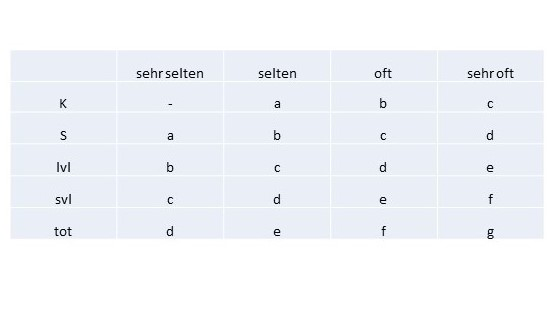
\includegraphics[width=12cm,height=7cm]{figures/Bewertungsskala}
		\caption[Bewertungsskala zur klassifizierung von Unfällen im urbanen Raum]{Bewertungsskala zur klassifizierung von Unfällen im urbanen Raum}\label{fig:Bewertungsskala}
	\end{figure}
\end{savenotes}

Zur besseren Veranschaulichung können die ermittelten Häufigkeiten mit Bezug zur jeweiligen Unfallschwere auch in einem Diagramm dargestellt werden. In Kapitel \ref{subsection:Risikoverteilung auf Unfalltypen} wurde vorgestellt wie \Textcite[S. 60]{Gschwendtner.2015} Unfalltypen anhand einer Risikoverteilung bewertet. So eine Risikoverteilung wird auch in dieser Arbeit verwendet. Hierfür wird auf der x-Achse die Häufigkeit angetragen, die Bereiche werden dabei entsprechend Tabelle \ref{tab:Haeufigkeits Bereiche} angepasst. Auf der y-Achse werden die fünf Unfallschweregrade, der Schwere nach aufsteigend, angegeben. Damit es auch hier möglich ist, die zugehörige Kritikalität abzulesen werden Risikoäquivalenten eingezeichnet. Den Bereichen zwischen den Risikoäquivalenten werden die gleichen Ordnungswerte wie in Abbildung \ref{fig:Bewertungsskala} zugeordnet. Abbildung \ref{fig:Bewertungsdiagramm} stellt ein Diagramm für die Bewertung der Unfalltypen ohne die Berücksichtigung der Kleinunfälle, Abbildung \ref{fig:Bewertungsdiagramm(2)} für die der Feintypen dar. Bei den gestrichelten Linien handelt es sich um die Risikoäquivalenten. Diese wurden anhand der vier Bereiche in Tabelle \ref{tab:Haeufigkeits Bereiche} ermittelt. Da die Bereiche für die Unfalltypen gleichmäßig gesplittet sind werden sie Anhand linearer Linien abgegrenzt. Die Bereiche für die Feintypen sind zur besseren Unterscheidung nicht gleichmäßig verteilt. Hierfür wurde über die Fixpunkte, welche in Tabelle \ref{tab:Haeufigkeits Bereiche} festgelegt werden, interpoliert um die Risikoäquivalenten zu erhalten. Die Fixpunkte wurden in den Abbildungen \ref{fig:Bewertungsdiagramm} und \ref{fig:Bewertungsdiagramm(2)} mit einem x gekennzeichnet. 

\begin{savenotes}
	\begin{figure}[H]
		\centering
		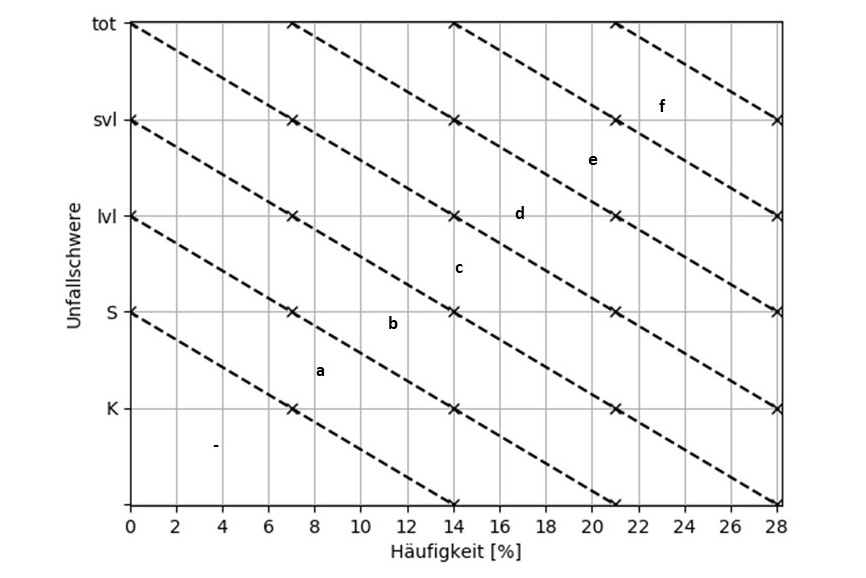
\includegraphics[width=10.5cm,height=7cm]{figures/Bewertungsdiagramm}
		\caption[Bewertungsdiagramm mit Risikoäquivalenten bei gleichmäßiger Verteilung der Häufigkeiten]{Bewertungsdiagramm mit Risikoäquivalenten bei gleichmäßiger Verteilung der Häufigkeiten}\label{fig:Bewertungsdiagramm}
	\end{figure}
\end{savenotes}

Ein Unfalltyp bzw. Feintyp kann aufgrund der unterschiedlichen Schweregrade bis zu fünf Mal bewertet werden. Sie kommen daher auch in der bildlichen Darstellung im Diagrammen häufiger vor. Maßgebend ist der Eintrag, dem die größte Ordnungsnummer zugeteilt wird und der somit das höchste Risiko mit sich bringt. Der Unfalltyp 7 kann z.B. einmal mit \enquote{b} aufgrund der Unfälle mit Leichtverletzten und einmal mit \enquote{d} aufgrund der Unfälle mit Sachschaden bewertet werden. Maßgeblich ist dann die höhere Ordnungsnummer \enquote{d}.

\begin{savenotes}
	\begin{figure}[H]
		\centering
		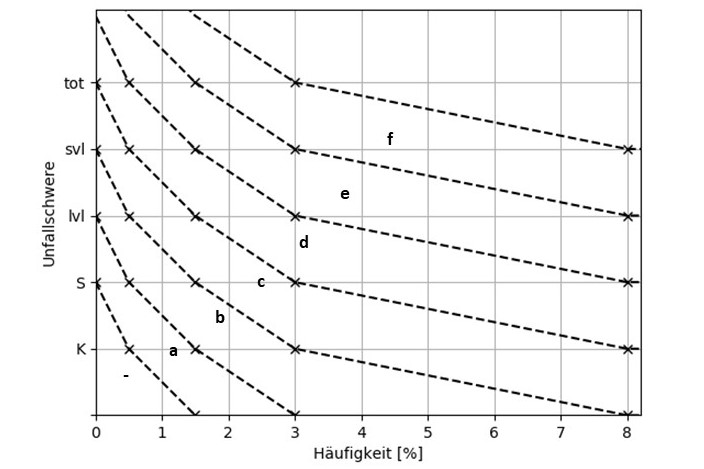
\includegraphics[width=10.5cm,height=7cm]{figures/Bewertungsdiagramm(2)}
		\caption[Bewertungsdiagramm mit Risikoäquivalenten bei ungleichmäßiger Verteilung der Häufigkeiten]{Bewertungsdiagramm mit Risikoäquivalenten bei ungleichmäßiger Verteilung der Häufigkeiten}\label{fig:Bewertungsdiagramm(2)}
	\end{figure}
\end{savenotes}


\subsection{Zuordnung von Unfällen zu urbanen Fahrsituationen}



%Hier schon die Skala Entwickeln und in Kapitel vier anwenden. Kapitel fünf kann dann wegfallen. Wie kommt man anhand der Unfalldaten von bestimmten Unfalltypen zu den Fahrsituationen?? Schritt für Schritt erklären.

%3. Den Fahrsituationen/Klassen die im Gebiet aufgenommen wurden wurden ebenfalls mögliche Feintypen zugeordnet. So ist es möglich kritische Situationen zu bestimmen. Wie kann man die Fahrsituationen vorstellen? Nur die kritischen nennen? Oder die Tabelle mit den Klassen und jeweiligen Feintypen einfach auch in den Anhang? Leser können allerdings mit den Nummern nichts anfangen. Also vllt doch nur die fünf bis 10 nennnen, die am kritischsten sind?
